\documentclass{FastFyp}
\usepackage{booktabs}
\usepackage{float}
\begin{document}
\newcommand{\supervisor}{Dr. Tahir Ejaz}
\newcommand{\university}{National University of Computer and Emerging Sciences, Lahore}
\newcommand{\fyptitle}{KisaanMadad: An Integrated Mobile Decision-Support System for Small-Scale Farmers in Punjab, Pakistan}
\newcommand{\degree}{BS}
\newcommand{\Studentone}{Zoraiz Anwar     22L-6998    BS(CS)}
\newcommand{\Studenttwo}{Ali Anzal     22L-6994    BS(CS)}
\newcommand{\Studentthree}{Naail Rayaan     22L-6755    BS(CS)}
\date{\today}
\renewcommand{\contentsname}{Table of Contents}

\makeatletter
    \begin{titlepage}
        
\includegraphics[width=0.2\linewidth]{Figures/nulogo.png}\hfill
        
\includegraphics[width=0.2\linewidth]{Figures/fast.png}\\
        \begin{center} 
            {\large\bfseries \university}\\[7ex]
            
\includegraphics[width=0.4\linewidth]{Figures/fastlogo.png}\\[8ex]
            {\huge \bfseries  \fyptitle }\\[10ex] 
            {\Studentone}\\{\Studenttwo}\\{\Studentthree}\\[4ex] 
            {Supervisor: \supervisor} \\ [10ex]
            {Final Year Project}\\
            {\large \@date}
        \end{center}
    \end{titlepage}    
\makeatother
\frontmatter

\newpage \thispagestyle{empty} \mbox{} \newpage %Aatira

\pagestyle{empty}  %Aatira
\section*{\begin{center}{Anti-Plagiarism Declaration} \end{center}} %Aatira
This is to declare that the above publication was produced under the:
\begin{flushleft}
\bf Title: \fyptitle
\end{flushleft}

is the sole contribution of the author(s), and no part hereof has been reproduced as it is the basis (cut and paste) that can be considered Plagiarism. All referenced parts have been used to argue the idea and cited properly. I/We will be responsible and liable for any consequence if a violation of this declaration is determined.
\\[4ex]
%% FYPTODO add the date and your names here
Date: ..........................

\begin{flushright}
Name: ..........................
\\[3ex]
Signature: ..........................
\\[6ex]
Name: ..........................
\\[3ex]
Signature: ..........................
\\[6ex]
Name: ..........................
\\[3ex]
Signature: ..........................

\end{flushright} 

\vspace{5 cm} %Aatira
 
\hrule %Aatira

\section*{Author's Declaration}
This states Authors’ declaration that the work presented in the report is their own, and has not been submitted/presented previously to any other institution or organization.
\pagebreak
% === ABSTRACT ===
\section*{Abstract}
Small-scale farmers in Pakistan face a confluence of structural challenges that severely constrain agricultural productivity and household income: acute water scarcity, persistent crop price volatility, and the near-total absence of data-driven decision-support tools accessible at the farm level. This report presents KisaanMadad (``Farmer Help''), an integrated mobile decision-support system designed for resource-constrained smallholders in Punjab, Pakistan. The system unifies four functionally distinct modules within a single cross-platform application: a probabilistic price forecasting engine employing a CNN-LSTM hybrid architecture benchmarked against Prophet and ARIMA baselines; a multi-criteria crop recommendation module that synthesises real-time weather, market proximity, planting calendars, and water availability; an irrigation scheduling engine grounded in the FAO-56 Penman-Monteith method, computing reference evapotranspiration $ET_0$ and applying crop-specific coefficients $K_c$ to derive field-level water requirements; and a financial planning toolkit comprising loan calculators, revenue projections, and expense tracking. All modules draw on localised data sources --- Punjab mandi price records from PAMRA and AMIS alongside meteorological inputs from the NASA POWER API --- and are presented through an Urdu-first interface to serve farmers with limited digital literacy. Collectively, KisaanMadad is expected to reduce the information asymmetry experienced by smallholders, improve irrigation efficiency, and provide actionable forecasts that enable more profitable and climate-resilient farming decisions.
\pagebreak
% === END ABSTRACT ===

% === EXECUTIVE SUMMARY ===
\section*{Executive Summary}

\paragraph{Background.}
Agriculture underpins Pakistan's economy, contributing 23.54\% to gross domestic product and employing 37.4\% of the national labour force \cite{pakistan_economic_survey_2025}. Yet the sector operates under severe structural stress. Approximately 97\% of Pakistani farmers own fewer than 12.5 acres of land \cite{rana2025farmers}, placing them squarely in the smallholder category where exposure to market shocks is highest and access to formal advisory services is lowest. Water insecurity compounds this vulnerability: per capita availability has collapsed from 5,260~m\textsuperscript{3} in 1951 to 908~m\textsuperscript{3} in 2021 --- below the internationally recognised scarcity threshold of 1,000~m\textsuperscript{3} \cite{pcrwr2021water} --- while irrigation efficiency across the canal network remains below 40\%. Price volatility driven by macroeconomic instability and strong commodity spillover effects further erodes farm income. Despite these pressures, the existing Pakistani agri-technology landscape remains fragmented: applications address either price discovery or weather information in isolation, and no reviewed solution integrates financial planning tools alongside agronomic advisory functions.

\paragraph{System Overview.}
KisaanMadad is a cross-platform mobile application targeting wheat, cotton, and rice cultivation in Punjab, Pakistan. It consolidates four decision-support modules into a unified, Urdu-language interface designed for farmers with limited digital literacy. The Price Forecasting module delivers probabilistic commodity price predictions for major Punjab mandi markets. The Crop Recommendation module generates ranked planting suggestions by scoring candidate crops against current weather conditions, market access, seasonal calendars, and water availability. The Irrigation Scheduling module produces weekly irrigation schedules tailored to a farmer's location, crop growth stage, and prevailing meteorological conditions. Finally, the Financial Planning module provides loan repayment calculators, crop revenue projections, and seasonal expense trackers --- functionality absent from all competing applications reviewed during this study.

\paragraph{Technical Approach.}
The price forecasting engine is built on a CNN-LSTM hybrid architecture, which exploits convolutional layers for local temporal pattern extraction and long short-term memory layers for longer-range dependency modelling. The model is trained on daily wholesale price records sourced from PAMRA and AMIS spanning 2018--2023 and benchmarked against Prophet and ARIMA baselines \cite{menculini2021comparing}. Irrigation scheduling is grounded in the FAO-56 Penman-Monteith standard \cite{allen1998crop}, computing reference evapotranspiration $ET_0$ from NASA POWER API solar radiation, temperature, and precipitation data, then multiplying by the appropriate crop coefficient $K_c$ to yield crop evapotranspiration $ET_c = K_c \times ET_0$; a Hargreaves--Samani fallback is applied when complete radiation data are unavailable. Crop recommendation scoring combines these meteorological inputs with FAO crop calendar data and proximity weighting for nearby mandis. The financial module employs rule-based calculators parameterised from user-provided inputs and prevailing crop revenue models.

\paragraph{Expected Outcomes and Novelty.}
KisaanMadad is expected to provide smallholder farmers with actionable, localised intelligence that reduces reliance on informal intermediaries (arthi) and mitigates the information asymmetry that currently characterises the mandi system. By embedding scientifically grounded irrigation scheduling directly on a mobile handset, the system aims to meaningfully improve on-farm water-use efficiency in a country facing acute water scarcity. Five principal contributions distinguish this work from the existing literature and commercial landscape: (1) it constitutes the first integrated platform to combine price forecasting, crop recommendation, irrigation scheduling, and financial planning within a single Pakistani agri-application; (2) it delivers FAO-56 compliant $ET_0$ computation on a mobile device for resource-constrained farmers with limited connectivity; (3) it introduces financial planning tools demonstrably absent from all reviewed existing solutions; (4) all models are trained and evaluated on localised PAMRA/AMIS mandi data and NASA POWER meteorological feeds rather than global commodity indices; and (5) the application is built with an Urdu-first interface, prioritising accessibility for the low-literacy smallholder population it serves.
\pagebreak
% === END EXECUTIVE SUMMARY ===


\pagestyle{fancy} %Aatira
\tableofcontents

\pagebreak
\listoffigures	% comment this if there are no figures
\addcontentsline{toc}{chapter}{List of Figures}
\pagebreak
\listoftables % comment this if there are no tables
\addcontentsline{toc}{chapter}{List of Tables}

\mainmatter


% === CHAPTER 1: INTRODUCTION ===
\chapter{Introduction}

Agriculture constitutes the backbone of Pakistan's economy, contributing 23.54\% to the national Gross Domestic Product (GDP) and employing 37.4\% of the country's total labour force \cite{pakistan_economic_survey_2025}. Despite this critical macroeconomic role, the sector is predominantly reliant on smallholder farmers, with 97\% of farmers owning less than 12.5 acres of land \cite{rana2025farmers}. These resource-constrained agriculturalists face profound systemic challenges that severely limit their productivity and profitability. Consequently, there remains a substantial yield gap of 40--60\% for major crops, such as wheat and sugarcane, when compared to the potential yields achieved in controlled research trials \cite{pbc2024agriculture}.

A primary driver of this agricultural underperformance is the intensifying water crisis. Pakistan's per capita water availability has precipitously declined from 5,260~m\textsuperscript{3} in 1951 to a critically low 908~m\textsuperscript{3} in 2021, falling below the internationally recognised water scarcity threshold of 1,000~m\textsuperscript{3} \cite{pcrwr2021water}. Compounding this scarcity is an acute lack of water management; overall irrigation efficiency remains below 40\%, and canal conveyance losses are estimated to reach approximately 38\% \cite{pcrwr2021water}. Furthermore, farmers' livelihoods are continuously threatened by extreme price volatility in local wholesale agricultural markets (\textit{mandis}), a phenomenon deeply exacerbated by macroeconomic instability and strong spillover effects between core commodities like wheat and rice \cite{habib2021price}. 

Although several agricultural technology solutions exist in the Pakistani market, they remain highly fragmented. Existing applications typically offer either weather forecasts or market prices in isolation, leaving a void for an integrated decision-support platform \cite{pasha2024agritech}. Most critically, none of the reviewed existing mobile solutions provide localised financial planning tools for smallholder farmers \cite{pasha2024agritech}. To address these pressing systemic issues, KisaanMadad is proposed as an integrated mobile decision-support system tailored for small-scale Pakistani farmers, aiming to bridge the information gap and promote sustainable, data-driven agricultural practices.

\section{Purpose of this Document}
The purpose of this document is to present the comprehensive design, implementation, and evaluation of KisaanMadad. In the face of fragmented existing solutions, KisaanMadad consolidates multiple disparate agricultural data streams into a unified, user-centric platform tailored for the specific needs of resource-constrained farmers in Punjab, Pakistan. Thus, the primary research question addressed by this project is whether an integrated, mobile-based decision-support system can effectively deliver localised crop recommendations, precise irrigation scheduling, accurate market price forecasting, and crucial financial planning directly to smallholder farmers. To answer this, the document details the development of the system's four core modules: ML-based Price Forecasting, multi-criteria Crop Recommendation, FAO-56 compliant Irrigation Scheduling, and rule-based Financial Planning.

\section{Intended Audience}
The primary intended audience for this document is the evaluation committee at the National University of Computer and Emerging Sciences (FAST-NUCES), Lahore, who will assess the technical rigour and academic contribution of the KisaanMadad Final Year Project. Additionally, the audience encompasses potential agricultural stakeholders, including government bodies like the Punjab Agriculture Marketing Regulatory Authority (PAMRA), non-governmental organisations, and agri-tech innovators. These entities will gain valuable insights into how integrating data-driven mobile technologies can empower small-scale farmers, optimise resource allocation, and enhance agricultural economic stability in Pakistan.

\section{Definitions, Acronyms, and Abbreviations}
Definitions of key terms, along with the expansions of acronyms and abbreviations used throughout this report, are provided below.

\subsection{Definitions}
\begin{description}
    \item[Mandi] A local wholesale agricultural market where crop trading and price determination occur.
    \item[Arthi] A middleman or commission agent operating within the mandi system, often facilitating transactions between farmers and buyers.
    \item[$ET_0$] Reference evapotranspiration, representing the environmental evaporative demand for a standard reference crop.
    \item[$K_c$] Crop coefficient, a standard value representing the physiological characteristics of a specific crop used to determine crop evapotranspiration.
    \item[FAO-56] The standard Penman-Monteith method for computing crop water requirements as outlined by the Food and Agriculture Organization \cite{allen1998crop}.
    \item[DSS] Decision-Support System, an information system that supports business or organisational decision-making activities.
    \item[Smallholder farmer] An agriculturalist owning or managing a small plot of land, typically less than 12.5 acres in the context of Pakistan, often constrained by limited resources.
\end{description}

\subsection{Acronyms and Abbreviations}
\begin{description}
    \item[PAMRA] Punjab Agriculture Marketing Regulatory Authority
    \item[AMIS] Agriculture Marketing Information Service
    \item[NASA POWER] NASA Prediction of Worldwide Energy Resources API
    \item[CNN-LSTM] Convolutional Neural Network and Long Short-Term Memory hybrid
    \item[FAO] Food and Agriculture Organization of the United Nations
    \item[DSS] Decision-Support System
    \item[FYP] Final Year Project
    \item[SDG] Sustainable Development Goal
\end{description}

\section{Conclusion}
To conclude, this chapter has provided a foundational understanding of the profound systemic challenges impeding Pakistan's agriculture sector, including severe water scarcity, widespread yield gaps, and significant market price volatility. The fragmented nature of current digital interventions necessitates the development of KisaanMadad, an integrated mobile decision-support system aimed at empowering smallholder farmers. The remaining document is structured to provide a comprehensive exploration of this proposed solution. Chapter 2 delves into an extensive literature review and analysis of related work. Chapter 3 discusses the system design and architecture of the proposed platform. Chapter 4 outlines the specific methodology employed for each of the four core modules. Chapter 5 details the technical implementation of the system. Chapter 6 presents the results and evaluation of the developed modules. Finally, Chapter 7 provides the conclusion and highlights avenues for future work.
% === END CHAPTER 1: INTRODUCTION ===
\chapter{Project Vision}

\section{Problem Domain Overview}
Agriculture constitutes 23.54\% of Pakistan's GDP and employs over a third of its workforce \cite{pakistan_economic_survey_2025}. However, an estimated 97\% of all farmers in Pakistan own and cultivate less than 12.5 acres of land \cite{rana2025farmers}, dominating the sector with smallholder operations that lack access to modern tools and data-driven insights. This productivity deficit results in severe yield gaps of 40-60\% \cite{adb2021pakistan}. Our integrated mobile application centralises essential agricultural decision-making processes---from crop selection and irrigation scheduling to price forecasting and financial planning. By deploying these modules collectively, the system ensures more reliable, timely, and actionable intelligence for farmers, ultimately enhancing both individual profitability and broader regional food security.

\section{Problem Statement}
The problem at hand involves the persistent reliance of Pakistani smallholder farmers on fragmented, traditional heuristics rather than integrated, data-driven tools. This deficiency results in suboptimal agricultural decisions across crop rotation, water utilisation, and market timing. By developing a unified, Urdu-first mobile decision-support system, we aim to automate complex predictive models and deliver actionable insights, thereby mitigating risks and improving overall farm efficiency.

\section{Problem Elaboration}
The overarching problem is characterised by several critical sub-domains that severely limit agricultural productivity and profitability.

\subsection{Market Information Asymmetry}
Smallholders face extreme price volatility and lack direct access to forward-looking, real-time wholesale mandi prices. Existing applications fail to provide predictive insights using advanced machine learning models (e.g., CNN-LSTM) \cite{pide2022wheat}, leaving farmers vulnerable to exploitation by intermediaries \cite{habib2021price} and unable to optimally time their sales.

\subsection{Irrigation Inefficiency}
Pakistan faces a severe hydrological crisis \cite{pcrwr2021water}, yet agricultural water use remains highly inefficient due to a reliance on traditional flood irrigation that causes massive volumetric waste \cite{worldbank2023water}. There is a distinct absence of accessible mobile tools that utilise scientifically validated evapotranspiration models, such as the FAO-56 standard \cite{allen1998crop}, to guide precise and efficient watering schedules.

\subsection{Fragmented Tools}
Current digital agricultural interventions are heavily siloed, offering discrete services like basic weather or isolated tips rather than a holistic platform \cite{pasha2024agritech}. Furthermore, these tools often feature complex English interfaces, making them largely inaccessible to the vast majority of rural farmers who require intuitive, Urdu-first design to overcome digital literacy barriers \cite{fao2023dss}.

\subsection{Financial Exclusion}
Smallholder farmers suffer from pervasive financial exclusion and a lack of formal planning capacity \cite{sbp2024finance}. The conspicuous absence of comprehensive financial modules in existing agri-tech applications heavily forces farmers to make critical livelihood decisions based purely on intuition rather than mathematically projected revenues, tracking inputs, and managing expenses.

\section{Goals and Objectives}
The goals and objectives of this project, addressing the lack of integrated decision-support for farmers, are as follows:
\begin{enumerate}
    \item Develop a probabilistic machine learning pipeline, benchmarking CNN-LSTM against baseline models \cite{menculini2021comparing}, to accurately forecast mandi crop prices.
    \item Implement a multi-criteria scoring algorithm for automated, localized crop recommendation.
    \item Design an irrigation scheduling module based on the FAO-56 Penman-Monteith standard for optimal water management.
    \item Engineer a comprehensive financial planning module for revenue projection and expense tracking.
    \item Deploy the system as an accessible, native Urdu-first mobile application.
\end{enumerate}

\section{Project Scope}
The project encompasses two distinct phases: the research phase and the development phase. The research phase involves a comprehensive literature review to gather insights on existing agricultural DSS, predictive modeling, and water management strategies. Additionally, it involves identifying reliable open-source data repositories, such as AMIS, PAMRA, and NASA POWER, that will serve as foundational inputs for our system.

The development phase focuses on creating the KisaanMadad platform, scoped geographically to Punjab, Pakistan, for wheat, cotton, and rice. The software encompasses four integrated modules: ML-based price forecasting, multi-criteria crop recommendation, FAO-56 compliant irrigation scheduling, and offline-capable financial calculators. The final deliverable is an Urdu-supported mobile application. Real-time physical IoT sensors, computer vision disease detection, and direct micro-lending integrations are strictly excluded from this scope.

\section{Sustainable Development Goals}
In this project, we are focusing on two specific SDGs: Zero Hunger, and Industry, Innovation, and Infrastructure.

\subsection{SDG 2: Zero Hunger}
\begin{figure}[htbp]
  \centering
  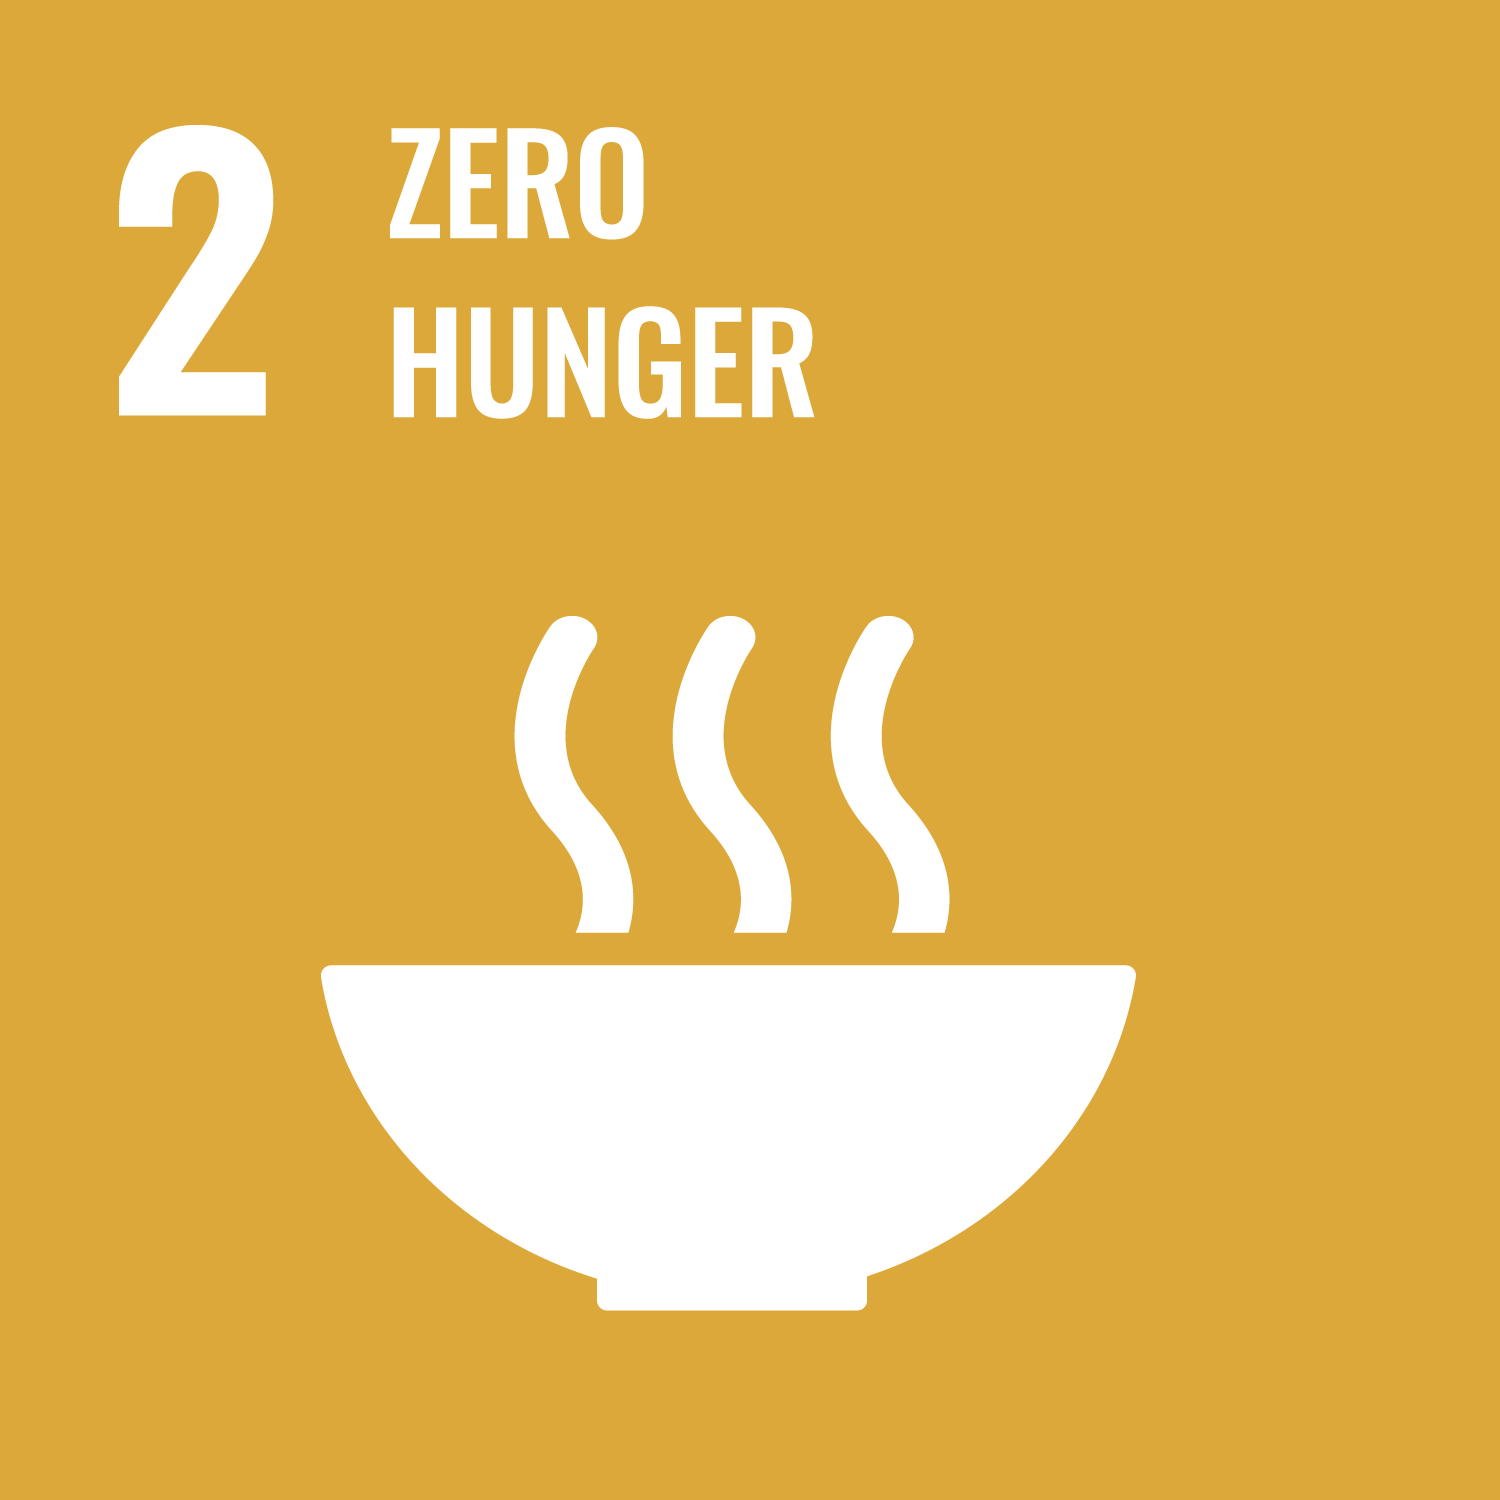
\includegraphics[width=0.4\linewidth]{Figures/sdg_2.png}
  \caption{United Nations Sustainable Development Goal 2: Zero Hunger.}
  \label{fig:sdg_2}
\end{figure}

The first SDG is Zero Hunger. By actively providing vulnerable rural farmers with transparent data-driven crop recommendations and sophisticated forward-looking price forecasts, the integrated system directly addresses foundational knowledge gaps. This project supports the goal of doubling the agricultural productivity and baseline incomes of small-scale food producers \cite{un2030agenda}, promoting resilient practices that adapt to climate change.

\subsection{SDG 9: Industry, Innovation, and Infrastructure}
\begin{figure}[htbp]
  \centering
  
\includegraphics[width=0.4\linewidth]{Figures/sdg_9.png}
  \caption{United Nations Sustainable Development Goal 9: Industry, Innovation, and Infrastructure.}
  \label{fig:sdg_9}
\end{figure}

The second SDG we address is Industry, Innovation, and Infrastructure. Our solution leverages innovative computational models---like CNN-LSTM forecasts and FAO-56 calculations \cite{allen1998crop}---and translates them into a highly accessible mobile interface. By doing so, we contribute to upgrading the fundamental technological capabilities of the agricultural sector, bridging the digital divide for rural workers without demanding prohibitive infrastructure investments \cite{un2030agenda}.

\section{Conclusion}
To conclude, this chapter establishes the foundational project vision by contextualising the profound challenges faced by smallholder farmers in Pakistan, including market volatility, water scarcity, and fragmented tools. By clearly articulating an unambiguous problem statement, identifying highly specific objectives, and formally defining the project scope, the chapter demonstrates how an integrated decision-support system can simultaneously advance critical UN Sustainable Development Goals and empower end-users. This sets the stage for a comprehensive exploration of our multifaceted approach in subsequent chapters.

\chapter{Literature Review / Related Work}

\section{Definitions, Acronyms and Abbreviations}

\subsection{Definitions}
\begin{description}
    \item[Evapotranspiration] The combined process of water loss from the earth's surface into the atmosphere through evaporation from soil and transpiration from plants.
    \item[Reference Evapotranspiration ($ET_0$)] The evapotranspiration rate from a well-watered reference surface, typically an extensive surface of green grass of uniform height.
    \item[Crop Coefficient ($K_c$)] A dimensionless ratio that relates the reference evapotranspiration to the actual crop evapotranspiration under standard conditions.
    \item[Mandi] A local or regional wholesale agricultural market where farmers sell their produce to commission agents or buyers.
    \item[Time Series Forecasting] The use of mathematical and statistical models to predict future values based on previously observed, chronologically ordered data.
    \item[Multi-Criteria Decision Making (MCDM)] A sub-discipline of operations research that explicitly evaluates multiple, often conflicting, criteria in decision making.
    \item[Soil Moisture] The quantity of water contained in the soil matrix, which is a critical variable for determining irrigation triggers.
    \item[Precision Agriculture] A farming management concept based on observing, measuring, and responding to inter- and intra-field variability in crops.
    \item[Vernacular Interface] A user interface localized into a native or indigenous language, tailored directly to users who do not speak English.
\end{description}

\subsection{Acronyms and Abbreviations}
\begin{description}
    \item[ANN] Artificial Neural Network
    \item[ARIMA] AutoRegressive Integrated Moving Average
    \item[CNN] Convolutional Neural Network
    \item[DSS] Decision Support System
    \item[ET\textsubscript{0}] Reference Evapotranspiration
    \item[FAO] Food and Agriculture Organization
    \item[GIS] Geographic Information System
    \item[LSTM] Long Short-Term Memory
    \item[MAE] Mean Absolute Error
    \item[MAPE] Mean Absolute Percentage Error
    \item[MCDM] Multi-Criteria Decision Making
    \item[ML] Machine Learning
    \item[NASA POWER] NASA Prediction of Worldwide Energy Resources
    \item[PAMRA] Punjab Agriculture Marketing Regulatory Authority
    \item[RMSE] Root Mean Square Error
    \item[UI] User Interface
    \item[UX] User Experience
\end{description}

\section{Detailed Literature Review}

\subsection{Agricultural Price Forecasting}

\subsubsection{Summary of the research items}
Menculini et al. \cite{menculini2021comparing} propose comparing deep learning methods such as Prophet alongside traditional ARIMA architectures for forecasting wholesale food prices. Using a large dataset of regional wholesale market prices, the study demonstrates that deep learning significantly outperforms classical statistical techniques, achieving lower error rates across different food commodity models.

In \cite{murugesan2022forecasting}, Murugesan and Mishra evaluate various deep learning architectures, including basic LSTM, bi-LSTM, stacked LSTM, and CNN-LSTM configurations, for predicting agricultural commodity prices. By extracting temporal sequences and spatial patterns, this study demonstrates that CNN-LSTM hybrids offer a highly accurate forecasting mechanism, outperforming basic recurrent neural networks in complex market scenarios.

The study by Joshi and Patel \cite{joshi2022cnn} utilized a CNN-Bidirectional LSTM approach specifically applied to price forecasting of volatile agricultural commodities in Gujarat. The bidirectional model effectively learned complex non-linear trading patterns, confirming the suitability of deep sequential models to capture both forward and backward temporal dependencies in local agriculture markets.

Finally, Habib et al. \cite{habib2021impact} analyses the impact of price volatility on agricultural commodities versus general food items with a specific focus on Pakistan. Utilizing localized economic datasets alongside historical prices, the authors demonstrate how macroeconomic instability and international commodity trends compound short-term price fluctuations. Their baseline findings underscore the necessity for robust, localized predictive tools to mitigate these shocks.

\subsubsection{Critical analysis of the research items}
The comparative study by Menculini et al. \cite{menculini2021comparing} successfully establishes the supremacy of deep learning over ARIMA; however, its reliance on stable European datasets limits its direct generalisability to highly erratic markets like Pakistan's mandi system. The deep learning models evaluated by Murugesan and Mishra \cite{murugesan2022forecasting} are notably powerful, yet complex architectures such as CNN-LSTM run the risk of overfitting when applied to data-scarce environments. The bidirectional approach from Joshi and Patel \cite{joshi2022cnn} handles long-term dependencies gracefully but lacks robust handling of exogenous variables, such as sudden policy shifts or extreme weather shocks, which regularly distort agricultural pricing. Meanwhile, Habib et al. \cite{habib2021impact} correctly identifies structural volatility issues in Pakistan's agriculture sector, but it remains heavily diagnostic rather than predictive, offering no implementable machine learning framework for regional stakeholders.

\subsubsection{Relationship to the proposed research work}
The CNN-LSTM architecture evaluated positively by Murugesan and Mishra \cite{murugesan2022forecasting} translates to the baseline design for KisaanMadad's price forecasting module, effectively balancing spatial feature extraction with time-series memory similar to the approach by Joshi and Patel \cite{joshi2022cnn}. To address the localized volatility highlighted by Habib et al. \cite{habib2021impact}, the module will rely on PAMRA and AMIS daily mandi price datasets spanning 2018--2023, rather than abstract global commodity curves. This bridges the gap between state-of-the-art deep learning findings and the resource-constrained needs of smallholder farmers in Pakistan's localized supply chains.

\subsubsection{Literature review summary table}
\begin{table}[htbp]
  \centering
  \caption{Literature review summary table for Agricultural Price Forecasting}
  \label{tab:price_forecasting}
  \begin{tabular}{p{0.15\linewidth} p{0.25\linewidth} p{0.25\linewidth} p{0.25\linewidth}}
    \toprule
    \textbf{Authors} & \textbf{Method} & \textbf{Results} & \textbf{Limitations} \\
    \midrule
    Murugesan \& Mishra \cite{murugesan2022forecasting} & CNN-LSTM and LSTM variants & Superiority of CNN-LSTM architectures & High computational cost, data heavy \\
    Joshi \& Patel \cite{joshi2022cnn} & CNN-Bidirectional LSTM & Accurate regional forecasting in Gujarat & Ignores exogenous market shocks \\
    Menculini et al. \cite{menculini2021comparing} & Prophet, Deep, ARIMA & Prophet and DL outperformed ARIMA & Tested on stable European datasets \\
    Habib et al. \cite{habib2021impact} & Economic Analysis & Identified severe structural price volatility & Diagnostic only, no predictive application \\
    \bottomrule
  \end{tabular}
\end{table}

\subsection{Crop Recommendation Systems}

\subsubsection{Summary of the research items}
Raghavendra et al. \cite{raghavendra2024systematic} present an extensive systematic literature review of machine learning algorithms utilized strictly for crop recommendation and yield estimation. Evaluating a consolidated body of work, the study demonstrates that ensemble methods and deep learning models consistently outperform traditional ML approaches when trained on diverse soil and atmospheric inputs.

In \cite{priyanka2023iot}, Priyanka et al. present an IoT-based crop recommendation framework using a machine learning backend for smart agriculture. Using sensory data measuring temperature and moisture, this study maps real-time environmental data to crop viability, demonstrating early success in automating recommendations dynamically.

Kancharagunta et al. \cite{kancharagunta2024crop} survey crop suitability systems by combining diverse IoT inputs with machine learning models. The survey highlights robust methodologies that integrate continuous environmental parameters into algorithmic decisions, successfully aiding both yield prediction and agricultural scheduling.

Finally, Apat et al. \cite{apat2023artificial} focuses specifically on artificial intelligence-based frameworks for crop guidance, proposing a lightweight intelligent recommendation system. By classifying secondary datasets encompassing soil and water availability features, the proposed system proves highly capable for farmers lacking expensive localized hardware.

\subsubsection{Critical analysis of the research items}
While Raghavendra et al. \cite{raghavendra2024systematic} provides an excellent foundational synthesis of machine learning in agriculture, the aggregated literature flattens regional heterogeneities, making perfect accuracy difficult to replicate in real-world scenarios. The IoT-driven architecture by Priyanka et al. \cite{priyanka2023iot} succeeds functionally but remains entirely cost-prohibitive for the mass majority of farmers owning under 12.5 acres. The survey approach by Kancharagunta et al. \cite{kancharagunta2024crop} confirms these hardware-adoption barriers. Conversely, the methodology by Apat et al. \cite{apat2023artificial} is a contextually robust software-only approach, yet its reliance on secondary static traces typically limits its predictive power against volatile precipitation cycles and climate changes.

\subsubsection{Relationship to the proposed research work}
KisaanMadad's crop recommendation system builds upon the software-centric philosophy presented by Apat et al. \cite{apat2023artificial} while aiming for the robust accuracy highlighted by Raghavendra et al. \cite{raghavendra2024systematic}. To overcome the lack of IoT hardware noted as a vulnerability by Priyanka et al. \cite{priyanka2023iot} and Kancharagunta et al. \cite{kancharagunta2024crop}, KisaanMadad will integrate dynamic, real-time meteorological inputs via the NASA POWER API alongside FAO crop calendars. By weighing continuous remote variables against static local criteria, KisaanMadad proposes an accurate recommendation system directly tailored to small-scale growers in Punjab.

\subsubsection{Literature review summary table}
\begin{table}[htbp]
  \centering
  \caption{Literature review summary table for Crop Recommendation Systems}
  \label{tab:crop_recommendation}
  \begin{tabular}{p{0.15\linewidth} p{0.25\linewidth} p{0.25\linewidth} p{0.25\linewidth}}
    \toprule
    \textbf{Authors} & \textbf{Method} & \textbf{Results} & \textbf{Limitations} \\
    \midrule
    Priyanka et al. \cite{priyanka2023iot} & IoT-based ML classification & High dynamic accuracy & Hardware-dependent, cost-prohibitive for smallholders \\
    Apat et al. \cite{apat2023artificial} & AI modeling on secondary data & Highly viable crop mapping & Relies heavily on static or prior weather traces \\
    Kancharagunta et al. \cite{kancharagunta2024crop} & Survey of ML/IoT systems & Synthesis of precision agritech adoption & Implementation complexity highlighted in survey \\
    Raghavendra et al. \cite{raghavendra2024systematic} & Systematic literature review & Identified optimal ensemble models & Generalised findings ignore regional variances \\
    \bottomrule
  \end{tabular}
\end{table}

\subsection{FAO-56 Irrigation Scheduling and ET\textsubscript{0} Estimation}

\subsubsection{Summary of the research items}
The foundational work by Allen et al. \cite{allen1998crop} establishes the global standard for computing crop water requirements via the FAO-56 Penman-Monteith method. This exhaustive procedural framework uses defined crop coefficients ($K_c$) and standard meteorological variables to produce the definitive reference evapotranspiration ($ET_0$) metric used globally.

In \cite{harris2025energy}, Harris proposes an energy-efficient smart irrigation framework combining edge AI with forecast-driven scheduling. By processing atmospheric variables against datasets like FAO and NASA POWER, the system efficiently minimized irrigation errors and operational costs through anticipatory remote sensing.

A study by Baber and Ullah \cite{baber2024short} evaluates the temperature-based Hargreaves-Samani equation against the standard FAO-56 Penman-Monteith equation for $ET_0$ estimation strictly within Pakistan. Using regional observatory data, this study demonstrates that while the PM method holds theoretical supremacy, the calibrated Hargreaves-Samani model is exceptionally suitable and accurate for data-scarce Pakistani regions.

Lastly, Jaafar et al. \cite{jaafar2022agsat} proposes AgSAT, a smart irrigation application reliant on cloud-fetched NASA POWER data combined with satellite imagery. By directly calculating daily crop ET and water requirements via remote methodologies, the authors demonstrate robust irrigation scheduling capabilities without physical ground equipment.

\subsubsection{Critical analysis of the research items}
The canonical methodology provided by Allen et al. \cite{allen1998crop} remains technically unmatched, yet its rigid demand for numerous meteorological variables makes it exceptionally difficult to directly deploy in sensor-less regions. The edge AI approach by Harris \cite{harris2025energy} brings powerful computation directly to farms but necessitates localized hardware or continuous connectivity. The regional evaluation by Baber and Ullah \cite{baber2024short} highlights a crucial compromise: the Hargreaves equation is simpler, but without proper calibration coefficients, farmers risk wasteful over-irrigation. The utilization of NASA POWER datasets by mobile applications like the one developed by Jaafar et al. \cite{jaafar2022agsat} presents an optimal software pathway, though resolution constraints inevitably restrict effectiveness on extreme micro-topographies.

\subsubsection{Relationship to the proposed research work}
Following the data sourcing successes of Harris \cite{harris2025energy} and Jaafar et al. \cite{jaafar2022agsat}, KisaanMadad bypasses physical hardware constraints by querying the NASA POWER API for real-time solar radiation and temperature. This remote data populates the core FAO-56 Penman-Monteith engine \cite{allen1998crop} compiled within the application. When wind speed or relative humidity inputs fail, KisaanMadad falls back to the temperature-driven Hargreaves methodology verified for use in local contexts by Baber and Ullah \cite{baber2024short}, guaranteeing uninterrupted irrigation scheduling.

\subsubsection{Literature review summary table}
\begin{table}[htbp]
  \centering
  \caption{Literature review summary table for FAO-56 Irrigation Scheduling}
  \label{tab:irrigation}
  \begin{tabular}{p{0.15\linewidth} p{0.25\linewidth} p{0.25\linewidth} p{0.25\linewidth}}
    \toprule
    \textbf{Authors} & \textbf{Method} & \textbf{Results} & \textbf{Limitations} \\
    \midrule
    Harris \cite{harris2025energy} & Edge AI and NASA POWER & Minimized energy load and water use & Requires continuous edge/cloud connectivity \\
    Baber \& Ullah \cite{baber2024short} & Penman-Monteith vs Hargreaves & Verified Hargreaves-Samani suitability & Calibration issues without proper coefficient setup \\
    Jaafar et al. \cite{jaafar2022agsat} & NASA POWER \& Satellite apps & Strong field-scale ET metrics & Satellite resolutions may overlook micro-climates \\
    Allen et al. \cite{allen1998crop} & FAO-56 foundational standard & Global ET0 benchmark established & Requires extensive meteorological input variables \\
    \bottomrule
  \end{tabular}
\end{table}

\subsection{Agricultural Mobile Applications in Developing Countries}

\subsubsection{Summary of the research items}
Kamal and Bablu \cite{kamal2023mobile} propose a systematic review regarding the widespread adoption of mobile applications by smallholder farmers operating in developing nations. Their analysis highlights how applications empowering farmers can accelerate agricultural development, provided digital payment systems and information delivery align with ground truths.

In \cite{amina2025factors}, Amina et al. specifically evaluate the factors influencing farmers' satisfaction and adoption of mobile phone applications for agricultural purposes within Faisalabad, Pakistan. The study found that usability and reliability directly determine satisfaction, pushing young farmers to optimize operations through reliable, well-designed mobile interfaces.

The investigation by Shahzad et al. \cite{shahzad2024mobile} examines digital agriculture adoption across Punjab, Pakistan, assessing the role of perceived awareness on farmer decisions. Utilizing a large random sample from diverse agroecological zones, the study proves that localized, culturally coherent outreach dramatically enhances platform adoption and overall digital proficiency.

Finally, examining existing Pakistani platforms, the Pasha \cite{pasha2024agritech} sector industry report reviews the state of agricultural tech solutions. The findings emphasize the systemic problem of fragmented single-utility tools, illustrating a severe market need for unified applications capable of managing multiple farming workflows simultaneously.

\subsubsection{Critical analysis of the research items}
The review by Kamal and Bablu \cite{kamal2023mobile} comprehensively diagnoses the positive macro-impacts but leaves technical implementation details, like offline caching or UI constraints, unaddressed. The regional usability analysis by Amina et al. \cite{amina2025factors} correctly identifies young farmers as the initial adoption catalyst in Pakistan, but overlooks the usability constraints faced by aging or low-literacy demographics. The Punjab-centric study by Shahzad et al. \cite{shahzad2024mobile} provides localized adoption data entirely relevant to KisaanMadad, yet highlights awareness, rather than purely technical features, as the core issue. Furthermore, the Pasha \cite{pasha2024agritech} sector report critically highlights app fragmentation, emphasizing that single-feature platforms fail to retain user interest without a comprehensive ecosystem backend.

\subsubsection{Relationship to the proposed research work}
Addressing the exact usability hurdles documented by Amina et al. \cite{amina2025factors} and the necessity of targeted local demographic awareness proven by Shahzad et al. \cite{shahzad2024mobile}, KisaanMadad is natively engineered with a vernacular Urdu User Interface utilizing accessible, heavily iconized navigational paradigms. Responding directly to the crippling fragmentation decried by the Pasha \cite{pasha2024agritech} report and following the empowerment guidelines set by Kamal and Bablu \cite{kamal2023mobile}, KisaanMadad consolidates price forecasting, crop recommendation, irrigation scheduling, and financial planning into one unified platform, representing a holistic, unprecedented counter to the limitations of current rural deployments.

\subsubsection{Literature review summary table}
\begin{table}[htbp]
  \centering
  \caption{Literature review summary table for Agricultural Mobile Applications}
  \label{tab:mobile_apps}
  \begin{tabular}{p{0.15\linewidth} p{0.25\linewidth} p{0.25\linewidth} p{0.25\linewidth}}
    \toprule
    \textbf{Authors} & \textbf{Method} & \textbf{Results} & \textbf{Limitations} \\
    \midrule
    Kamal \& Bablu \cite{kamal2023mobile} & Review of agricultural dev apps & Proven tech empowerment linkages & Diagnoses macro trends without UI technical guidance \\
    Amina et al. \cite{amina2025factors} & Faisalabad adoption survey & Identified reliability as key driver & Predominantly evaluates younger demographics \\
    Shahzad et al. \cite{shahzad2024mobile} & Punjab field adoption stats & Strong correlation with local awareness & Awareness-centric, lacks focus on app mechanics \\
    Pasha \cite{pasha2024agritech} & Industry sector reporting & Identified severe app fragmentation & Enterprise focus, no underlying predictive models \\
    \bottomrule
  \end{tabular}
\end{table}

\subsection{Related Applications}

\subsubsection{Summary of the research items}
The Kisan App \cite{kisanapp2024} is an established digital advisory platform targeting farmers primarily within Punjab, Pakistan. It focuses heavily on static farming methodologies, regional news alerts, and general weather reporting. It boasts a large user base due to widespread government and telco collaboration, effectively serving as an elementary portal for regional agricultural information.

Farmdar \cite{farmdar2024} is an established agritech business offering a suite of B2B products (such as CropScan and Yield Pro) rather than a single farmer-facing application. It employs high-resolution, multi-spectral remote sensing AI over satellite imagery to monitor crop health at scale. Deployed heavily across sugar mills, corporate farms, and lending institutions throughout Pakistan and globally, it specializes in actionable spatial detection regarding nutrient deficiencies, pest outbreaks, and yield predictions, driven directly by precision GIS analytics.

BaKhabar Kissan \cite{bakhabarkissan2024} is undoubtedly Pakistan's most prominent holistic agricultural advisory platform. Supported by a robust backend call-center infrastructure and an aggressive telecommunications partnership, the application delivers localized weather parameters, pest warnings, and up-to-date regional market commodity prices. It caters extensively to smallholder farmers seeking daily operational guidance.

\subsubsection{Critical analysis of the research items}
While the Kisan App \cite{kisanapp2024} is accessible, its feature set is profoundly rudimentary; it severely lacks any advanced machine learning integration for intelligent crop recommendations, and it does not possess price forecasting or financial calculators, rendering it purely informational rather than a true decision support system. Farmdar \cite{farmdar2024} leverages state-of-the-art spatial precision, yet its enterprise focus, B2B product structure, and heavy reliance on extensive land tracts organically alienate the 97\% of farmers confined to holdings under 12.5 acres. Conversely, BaKhabar Kissan \cite{bakhabarkissan2024} addresses smallholders effectively through price reporting, but critically acts only as a diagnostic repository; it fails entirely to forecast incoming price volatility, offers no sophisticated FAO-56 integrated localized irrigation scheduling, and completely omits modular financial planning.

\subsubsection{Relationship to the proposed research work}
The gap analysis of existing entities inherently cements KisaanMadad's unique technological positioning. While BaKhabar Kissan \cite{bakhabarkissan2024} provides basic prices, KisaanMadad introduces dynamic models predicting future prices \cite{murugesan2022forecasting} previously unavailable at zero cost. Unlike the enterprise-focused Farmdar products \cite{farmdar2024}, KisaanMadad explicitly targets smallholders by replacing cost-prohibitive remote B2B analytics with multi-criteria recommendations and FAO-56 \cite{allen1998crop} frameworks operating natively on mobile. Finally, surpassing the passive information structures of the Kisan App \cite{kisanapp2024}, KisaanMadad is the first architecture to fuse agronomic tools with foundational financial planning resources, closing the loop between ecological farm management and smallholder macroeconomic survival.

\subsubsection{Related applications summary table}
\begin{table}[ht]
  \centering
  \caption{Related applications summary table}
  \label{tab:related_apps}
  \begin{tabular}{p{0.15\linewidth} p{0.30\linewidth} p{0.30\linewidth} p{0.15\linewidth}}
    \toprule
    \textbf{Application} & \textbf{Features} & \textbf{Relevance to KisaanMadad} & \textbf{Limitations} \\
    \midrule
    Kisan App \cite{kisanapp2024} & News, static advice, weather & General template for UI accessibility & No ML, no forecasting, no financial tools \\
    Farmdar \cite{farmdar2024} & Remote sensing B2B products & Demonstrates success of precision agritech & Expensive, enterprise-focused, not a direct consumer app \\
    BaKhabar Kissan \cite{bakhabarkissan2024} & Daily prices, pest warnings, call centre & Key competitor in price dissemination & Passive reporting only, no FAO-56 irrigation \\
    \bottomrule
  \end{tabular}
\end{table}

\pagebreak
 
% === CHAPTER 4: SRS ===
\chapter{Software Requirements Specification}

This chapter outlines the Software Requirements Specification (SRS) for the KisaanMadad integrated mobile decision-support system. It presents the core features, formal functional and non-functional requirements, quality attributes, system constraints, use cases, and database design necessary for deployment in a resource-constrained agricultural environment.

\section{List of Features}

The system provides the following primary features:
\begin{itemize}
    \item Probabilistic mandi price forecasting with confidence intervals
    \item Multi-criteria crop recommendation engine
    \item FAO-56 compliant irrigation scheduling with NASA POWER integration
    \item Loan calculator and revenue projection tools
    \item Expense tracker
    \item Urdu language interface
    \item Offline-capable core functionality
    \item Push notifications for price alerts
\end{itemize}

\section{Functional Requirements}

\subsection{Price Forecasting Module}
\begin{enumerate}
    \item The system \textbf{shall} allow the Farmer to choose a primary crop (wheat, cotton, or rice) and generate a 30-day probabilistic mandi price forecast.
    \item The system \textbf{shall} retrieve historical daily PAMRA and AMIS records to base its forecasting algorithm outputs.
    \item The system \textbf{shall} display the corresponding upper and lower confidence intervals alongside the median predicted price chart.
    \item The system \textbf{shall} trigger push notifications if an anomaly or significant 10\% short-term price jump is detected for the Farmer's subscribed crop.
\end{enumerate}

\subsection{Crop Recommendation Module}
\begin{enumerate}
    \item The system \textbf{shall} accept explicit input parameters from the Farmer including land size, district, and planting season.
    \item The system \textbf{shall} process these geographic parameters via the NASA POWER API to retrieve historical and real-time localized weather data.
    \item The system \textbf{shall} evaluate inputs systematically against established FAO crop calendars and aggregate environmental metrics.
    \item The system \textbf{shall} calculate and output a multi-criteria compatibility score representing the suitability of the top recommended crops.
\end{enumerate}

\subsection{Irrigation Scheduling Module}
\begin{enumerate}
    \item The system \textbf{shall} implement the standard FAO-56 Penman-Monteith method to derive baseline reference evapotranspiration ($ET_0$).
    \item The system \textbf{shall} parse real-time solar radiation, temperature, and precipitation factors directly from the NASA POWER API payload.
    \item The system \textbf{shall} apply the designated crop coefficient ($K_c$) dynamically aligned with the Farmer's active crop growth cycle to determine crop evapotranspiration ($ET_c$).
    \item The system \textbf{shall} generate an actionable irrigation schedule detailing required water volume or watering durations.
\end{enumerate}

\subsection{Financial Planning Module}
\begin{enumerate}
    \item The system \textbf{shall} feature an interactive loan calculator requiring interest rate, principal amount, and total tenure to compute uniform monthly installments.
    \item The system \textbf{shall} process an expected yield input from the Farmer combined with current mandi trading rates to formulate projected revenue.
    \item The system \textbf{shall} allow the Farmer to record individual input overheads such as seed, fertilizer, and transport costs into an expense tracker.
    \item The system \textbf{shall} automatically derive and present a projected gross margin comparing accrued tracking expenses against formulated revenues.
\end{enumerate}

\subsection{Authentication and User Management}
\begin{enumerate}
    \item The system \textbf{shall} allow the Farmer to register a distinct account utilizing their mobile number and standard OTP token confirmation.
    \item The system \textbf{shall} require the Farmer to populate an initial profile detailing primary farm district and language interface preference.
    \item The system \textbf{shall} securely store established Farmer profile data locally and synchronize passively to the cloud backend.
\end{enumerate}

\section{Quality Attributes}

\begin{table}[htbp]
  \centering
  \caption{System Quality Attributes}
  \label{tab:quality_attributes}
  \begin{tabular}{@{}p{0.2\linewidth} p{0.4\linewidth} p{0.3\linewidth}@{}}
    \toprule
    \textbf{Quality Attribute} & \textbf{Description} & \textbf{Relevance to KisaanMadad} \\
    \midrule
    Performance & How rapidly the system resolves functions and loads screens. & Critical for acceptable price forecast loading. \\
    Reliability & Operational continuity free from unexpected errors. & Vital for daily irrigation scheduling reliability. \\
    Usability & Clarity and operational ease of the user interface. & Requires Urdu, icons, and non-complex structural design. \\
    Availability & Consistency of application and backend accessibility. & Necessitates offline resilience in rural Punjab. \\
    Scalability & Capability to expand user bases and data payloads. & Adapts to expanding PAMRA archives and Farmer registrations. \\
    Maintainability & Ease of subsequent application modification and patching. & Allows systematic swapping of evolving inference models. \\
    Portability & Environmental independence for multi-device execution. & Achieved utilizing cross-platform mobile frameworks. \\
    \bottomrule
  \end{tabular}
\end{table}

\section{Non-Functional Requirements}

\subsection{Performance}
\begin{itemize}
    \item The price forecast query execution \textbf{shall} complete and return graphic visuals within 3 seconds maximum on a standard 3G/4G cellular network.
    \item The application \textbf{shall} present core features using offline local cache instantly under scenarios with zero active connectivity.
\end{itemize}

\subsection{Usability}
\begin{itemize}
    \item The UI \textbf{shall} integrate a fully functional vernacular Urdu framework employing familiar iconography to accommodate low-literacy farmers.
    \item The application interface \textbf{shall} limit navigational depth, ensuring any singular core feature is accessible within a maximum of 3 taps from the Home Dashboard.
    \item On-screen visual elements and typefaces \textbf{shall} remain completely legible on conventional 5-inch low-resolution Android display panels.
\end{itemize}

\subsection{Reliability}
\begin{itemize}
    \item The overarching API services layer \textbf{shall} maintain an uptime target of 99.9\% throughout critical regional harvesting months.
    \item The system \textbf{shall} implement graceful degradation, switching automatically to the Hargreaves protocol utilizing local historical temperatures if NASA POWER API endpoints become unresponsive.
\end{itemize}

\subsection{Security}
\begin{itemize}
    \item The system \textbf{shall} preserve stringent Farmer data privacy policies, collecting zero arbitrary Personally Identifiable Information (PII) without transparent and explicit digital consent.
    \item All external and internal backend network transmissions \textbf{shall} strictly utilize encrypted TLS implementations by default.
\end{itemize}

\section{Assumptions}

\begin{enumerate}
    \item The Farmer possesses internet connectivity initially to accommodate application download and primary agricultural data synchronization.
    \item The deployment environment consists of low to mid-range Android smartphones running a minimum OS version of Android 8.0.
    \item Continuous and un-throttled availability of the external NASA POWER API data payloads is granted during query cycles.
    \item Key government and public sources like PAMRA and AMIS will persistently offer stable historic market pricing for the core commodities in Punjab.
    \item The Farmer exhibits a baseline level of smartphone operational literacy required to manipulate touchscreen interfaces.
    \item Data pulled via longitude and latitude coordinate boundaries from NASA matches the respective farm's atmospheric microclimate with minimal deviation.
\end{enumerate}

\section{Use Cases}

\begin{table}[htbp]
  \centering
  \caption{Use Case: View Price Forecast}
  \label{uc:view_forecast}
  \begin{tabular}{|p{0.3\linewidth}|p{0.65\linewidth}|}
    \hline
    \textbf{Name} & View Price Forecast \\
    \hline
    \textbf{Actors} & Farmer \\
    \hline
    \textbf{Summary} & Farmer accesses a projected moving price trend for an agricultural commodity. \\
    \hline
    \textbf{Pre-Conditions} & Appropriate models are cached; UI is operational. \\
    \hline
    \textbf{Post-Conditions} & Forecast graph visually highlights predictions and intervals. \\
    \hline
    \textbf{Special Requirements} & The chart visualizes a clear median trend surrounded by intervals. \\
    \hline
    \multicolumn{2}{|c|}{\textbf{Basic Flow}} \\
    \hline
    \textbf{Actor Action} & \textbf{System Response} \\
    \hline
    1. Selects desired crop icon & 2. Prompts ML model for predictive matrices \\
    & 3. Plots timeline chart and upper/lower arrays \\
    \hline
    \multicolumn{2}{|c|}{\textbf{Alternative Flow}} \\
    \hline
    \multicolumn{2}{|p{0.95\linewidth}|}{2a. If local time-series data is stale, the app pushes an alert guiding the user to connect and refresh the cached history prior to execution.} \\
    \hline
  \end{tabular}
\end{table}

\begin{table}[htbp]
  \centering
  \caption{Use Case: Get Crop Recommendation}
  \label{uc:get_crop_rec}
  \begin{tabular}{|p{0.3\linewidth}|p{0.65\linewidth}|}
    \hline
    \textbf{Name} & Get Crop Recommendation \\
    \hline
    \textbf{Actors} & Farmer \\
    \hline
    \textbf{Summary} & Input localized metrics to receive ranked crop suggestions. \\
    \hline
    \textbf{Pre-Conditions} & The device possesses network authority to fetch NASA POWER parameters. \\
    \hline
    \textbf{Post-Conditions} & Screen enumerates recommended crops by descending score. \\
    \hline
    \textbf{Special Requirements} & Employs FAO crop calendars internally. \\
    \hline
    \multicolumn{2}{|c|}{\textbf{Basic Flow}} \\
    \hline
    \textbf{Actor Action} & \textbf{System Response} \\
    \hline
    1. Inputs land acres and regional district & 2. Gathers constraints and invokes scoring mechanism \\
    & 3. Returns the formulated and ranked list to the display \\
    \hline
    \multicolumn{2}{|c|}{\textbf{Alternative Flow}} \\
    \hline
    \multicolumn{2}{|p{0.95\linewidth}|}{2a. If explicit geographical location polling fails, the UI requests manual district confirmation before proceeding.} \\
    \hline
  \end{tabular}
\end{table}

\begin{table}[htbp]
  \centering
  \caption{Use Case: Generate Irrigation Schedule}
  \label{uc:get_irrigation}
  \begin{tabular}{|p{0.3\linewidth}|p{0.65\linewidth}|}
    \hline
    \textbf{Name} & Generate Irrigation Schedule \\
    \hline
    \textbf{Actors} & Farmer \\
    \hline
    \textbf{Summary} & Determine temporal watering cycles via FAO-56. \\
    \hline
    \textbf{Pre-Conditions} & Farmer specifies identical active crop phase and planting baseline. \\
    \hline
    \textbf{Post-Conditions} & System delivers specific watering periods or volume suggestions. \\
    \hline
    \textbf{Special Requirements} & Real-time precision of evapotranspiration calculations. \\
    \hline
    \multicolumn{2}{|c|}{\textbf{Basic Flow}} \\
    \hline
    \textbf{Actor Action} & \textbf{System Response} \\
    \hline
    1. Taps on Irrigation module & 2. Validates crop and parses NASA POWER weather objects \\
    3. Confirms operation & 4. Resolves Penman-Monteith equation and produces the calendar \\
    \hline
    \multicolumn{2}{|c|}{\textbf{Alternative Flow}} \\
    \hline
    \multicolumn{2}{|p{0.95\linewidth}|}{4a. Unreachable NASA endpoints systematically divert calculation pathways to utilize local historical extrema variables against the Hargreaves method.} \\
    \hline
  \end{tabular}
\end{table}

\begin{table}[htbp]
  \centering
  \caption{Use Case: Calculate Loan / Revenue Projection}
  \label{uc:finance_tools}
  \begin{tabular}{|p{0.3\linewidth}|p{0.65\linewidth}|}
    \hline
    \textbf{Name} & Calculate Loan / Revenue Projection \\
    \hline
    \textbf{Actors} & Farmer \\
    \hline
    \textbf{Summary} & Assess future revenue potentials or amortized banking loan structures. \\
    \hline
    \textbf{Pre-Conditions} & Up-to-date mandi prices are downloaded within the local state space. \\
    \hline
    \textbf{Post-Conditions} & Mathematical integers translate to presented financial layouts. \\
    \hline
    \textbf{Special Requirements} & The interface reflects numeric integers efficiently and cleanly. \\
    \hline
    \multicolumn{2}{|c|}{\textbf{Basic Flow}} \\
    \hline
    \textbf{Actor Action} & \textbf{System Response} \\
    \hline
    1. Accesses Financial tools pane & 2. Presents dual isolated modes \\
    3. Triggers Revenue slider element & 4. Multiplies expected yield by mandi constants live \\
    \hline
    \multicolumn{2}{|c|}{\textbf{Alternative Flow}} \\
    \hline
    \multicolumn{2}{|p{0.95\linewidth}|}{3a. If the Farmer interacts with the Loan array, the module requests Principal, Interest rate constraints to formulate the cyclic installment value instantly.} \\
    \hline
  \end{tabular}
\end{table}

\begin{table}[htbp]
  \centering
  \caption{Use Case: Set Up Farmer Profile}
  \label{uc:setup_profile}
  \begin{tabular}{|p{0.3\linewidth}|p{0.65\linewidth}|}
    \hline
    \textbf{Name} & Set Up Farmer Profile \\
    \hline
    \textbf{Actors} & Farmer \\
    \hline
    \textbf{Summary} & Initializing the application state parameters corresponding to user specifics. \\
    \hline
    \textbf{Pre-Conditions} & The primary OTP handshake sequence has concluded. \\
    \hline
    \textbf{Post-Conditions} & An active profile is structured within standard DB formats. \\
    \hline
    \textbf{Special Requirements} & Non-intrusive collection of PII. \\
    \hline
    \multicolumn{2}{|c|}{\textbf{Basic Flow}} \\
    \hline
    \textbf{Actor Action} & \textbf{System Response} \\
    \hline
    1. Submits localized preferences & 2. Translates object states to persistent localized caching \\
    & 3. Synchronizes background sequence to corresponding remote records \\
    \hline
    \multicolumn{2}{|c|}{\textbf{Alternative Flow}} \\
    \hline
    \multicolumn{2}{|p{0.95\linewidth}|}{3a. Application is entirely offline; local states update identically and cloud push cycles are suspended pending affirmative connectivity pulses.} \\
    \hline
  \end{tabular}
\end{table}

\begin{table}[htbp]
  \centering
  \caption{Use Case: Switch Language to Urdu}
  \label{uc:switch_urdu}
  \begin{tabular}{|p{0.3\linewidth}|p{0.65\linewidth}|}
    \hline
    \textbf{Name} & Switch Language to Urdu \\
    \hline
    \textbf{Actors} & Farmer \\
    \hline
    \textbf{Summary} & Transitions application terminology formats into native Urdu representations. \\
    \hline
    \textbf{Pre-Conditions} & Preloaded typography assets exist inside the host bundle. \\
    \hline
    \textbf{Post-Conditions} & Total systematic transition of interface architecture text boundaries. \\
    \hline
    \textbf{Special Requirements} & Responsive Right-to-Left (RTL) matrix manipulation logic. \\
    \hline
    \multicolumn{2}{|c|}{\textbf{Basic Flow}} \\
    \hline
    \textbf{Actor Action} & \textbf{System Response} \\
    \hline
    1. Chooses specific language toggle & 2. Injects configuration flags across rendering states \\
    & 3. Restarts navigational layout matrix aligned RTL in Urdu \\
    \hline
    \multicolumn{2}{|c|}{\textbf{Alternative Flow}} \\
    \hline
    \multicolumn{2}{|p{0.95\linewidth}|}{3a. In circumstances lacking explicitly translated keys, the rendering module conservatively inherits standard icon-driven or English fallbacks to prohibit blank rendering zones.} \\
    \hline
  \end{tabular}
\end{table}

\section{Hardware and Software Requirements}

\subsection{Hardware Requirements}
Deployment architecture demands an introductory-level low-budget Android smartphone possessing a baseline of 2GB operative RAM and 500MB storage capacity to isolate essential model artifacts and dataset caching. The system anticipates intermittent, yet unavoidable, network communication to synchronize historic elements. The backend service instances operate on server architectures characterized by high-concurrency capability, optimized compute resources, and rapid multi-threaded I/O environments.

\subsection{Software Requirements}

\begin{table}[htbp]
  \centering
  \caption{Software Component and Technology Justification}
  \label{tab:sw_requirements}
  \begin{tabular}{@{}p{0.25\linewidth} p{0.25\linewidth} p{0.45\linewidth}@{}}
    \toprule
    \textbf{Component} & \textbf{Technology Choice} & \textbf{Justification} \\
    \midrule
    Mobile Frontend & Flutter & Employs an efficient cross-platform foundation producing a unified Android/iOS artifact optimally structured for rural settings~\cite{khan2023cross}. \\
    Backend API & FastAPI (Python) & Asynchronous lightweight Python framework explicitly resolving overhead latency bridging native ML execution environments~\cite{patel2023fastapi}. \\
    Price Forecasting Model & CNN-LSTM & Deep learning algorithms effectively surpassing traditional methods corresponding to high-volatility agricultural modeling sequences~\cite{habib2021price, ahmed2022lstm}. \\
    Irrigation Module & FAO-56 + NASA POWER API & Integrating undisputed international standards~\cite{allen1998crop} reinforced by verified reanalysis parameters~\cite{silva2022nasapower}. \\
    Database & PostgreSQL & Relational rigidity perfectly handling complex indexing essential to aggregate time-series financial information successfully~\cite{singh2021agridb}. \\
    ML Model Serving & TensorFlow Lite & Condenses complex models to minimal proportions necessary for executing localized offline inferences natively~\cite{patel2023fastapi}. \\
    Language Support & Flutter i18n + Urdu font & Crucial resolution for surmounting the fundamental adoption barriers characteristic of low-literacy South Asian regions~\cite{raza2021urduui}. \\
    \bottomrule
  \end{tabular}
\end{table}

\section{Graphical User Interface}

Initial spatial constraints formulated over the foundational interactive screens intended for the KisaanMadad platform.

\begin{figure}[htbp]
  \centering
  \fbox{\rule{0pt}{5cm}\rule{0.7\linewidth}{0pt}}
  \caption{Wireframe: Home Dashboard}
  \label{fig:wf_home}
\end{figure}

\begin{figure}[htbp]
  \centering
  \fbox{\rule{0pt}{5cm}\rule{0.7\linewidth}{0pt}}
  \caption{Wireframe: Price Forecast Screen}
  \label{fig:wf_forecast}
\end{figure}

\begin{figure}[htbp]
  \centering
  \fbox{\rule{0pt}{5cm}\rule{0.7\linewidth}{0pt}}
  \caption{Wireframe: Crop Recommendation Screen}
  \label{fig:wf_croprec}
\end{figure}

\begin{figure}[htbp]
  \centering
  \fbox{\rule{0pt}{5cm}\rule{0.7\linewidth}{0pt}}
  \caption{Wireframe: Irrigation Schedule Screen}
  \label{fig:wf_irrig}
\end{figure}

\begin{figure}[htbp]
  \centering
  \fbox{\rule{0pt}{5cm}\rule{0.7\linewidth}{0pt}}
  \caption{Wireframe: Financial Tools Screen}
  \label{fig:wf_finance}
\end{figure}

\begin{figure}[htbp]
  \centering
  \fbox{\rule{0pt}{5cm}\rule{0.7\linewidth}{0pt}}
  \caption{Wireframe: Language Settings Screen}
  \label{fig:wf_language}
\end{figure}

\section{Database Design}

\subsection{ER Diagram}
The relational database topography fundamentally establishes \textbf{Farmer} as the core pivot entity directly corresponding to various secondary elements. A singular \textbf{Farmer} entity initiates a one-to-many link resolving downstream active \textbf{Crop} entities. Expanding horizontally, a registered \textbf{Crop} associates directly with daily chronological \textbf{MandiPrice} fluctuations while similarly mapping calculated \textbf{IrrigationSchedule} records. Abstract elements like \textbf{WeatherData} iterate asynchronously. Furthermore, granular financial operations spawn \textbf{LoanRecord} and \textbf{ExpenseRecord} parameters which fold linearly backward in many-to-one aggregation mapping to the original \textbf{Farmer} identifier.

\subsection{Data Dictionary}

\begin{table}[htbp]
  \centering
  \caption{Data Dictionary: Farmer Entity}
  \label{tab:dict_farmer_table}
  \begin{tabular}{@{}p{0.2\linewidth} p{0.2\linewidth} p{0.25\linewidth} p{0.25\linewidth}@{}}
    \toprule
    \textbf{Attribute} & \textbf{Data Type} & \textbf{Constraints} & \textbf{Description} \\
    \midrule
    farmer\_id & UUID & PRIMARY KEY & Distinct internal account token \\
    phone\_number & VARCHAR(15) & UNIQUE, NOT NULL & Formatted active MSISDN string \\
    name & VARCHAR(100) & - & Alphabetical title sequence \\
    location\_lat & FLOAT & - & GPS geographic latitude parameter \\
    location\_long & FLOAT & - & GPS geographic longitude parameter \\
    farm\_size & DECIMAL(5,2) & $> 0$ & Quantitative acreage domain \\
    pref\_language & VARCHAR(10) & DEFAULT 'UR' & Selected locale (UR/EN) \\
    \bottomrule
  \end{tabular}
\end{table}

\begin{table}[htbp]
  \centering
  \caption{Data Dictionary: MandiPrice Entity}
  \label{tab:dict_mandi_table}
  \begin{tabular}{@{}p{0.2\linewidth} p{0.2\linewidth} p{0.25\linewidth} p{0.25\linewidth}@{}}
    \toprule
    \textbf{Attribute} & \textbf{Data Type} & \textbf{Constraints} & \textbf{Description} \\
    \midrule
    price\_id & SERIAL & PRIMARY KEY & Index sequential reference \\
    crop\_name & VARCHAR(50) & NOT NULL & Textual specific commodity \\
    mandi\_loc & VARCHAR(100) & NOT NULL & Active geographic trading zone \\
    record\_date & DATE & NOT NULL & Historical archival chronological stamp \\
    min\_price & DECIMAL(8,2) & - & Lowest formulated boundary mark \\
    max\_price & DECIMAL(8,2) & - & Highest formulated boundary mark \\
    avg\_price & DECIMAL(8,2) & NOT NULL & Arithmetic aggregated trading index \\
    \bottomrule
  \end{tabular}
\end{table}

\section{Risk Analysis}

\begin{table}[htbp]
  \centering
  \caption{Project Risk Configuration}
  \label{tab:risk_table}
  \begin{tabular}{@{}p{0.25\linewidth} p{0.15\linewidth} p{0.1\linewidth} p{0.1\linewidth} p{0.3\linewidth}@{}}
    \toprule
    \textbf{Risk} & \textbf{Type} & \textbf{Likelihood} & \textbf{Impact} & \textbf{Mitigation Strategy} \\
    \midrule
    NASA POWER API downtime & Technical & Medium & High & Retain fallback methods mirroring the Hargreaves protocol executing independently over cached averages. \\
    PAMRA data gaps & Data & High & Medium & Design processing mechanisms configured to resolve non-sequential blanks via structural interpolation matrices. \\
    Low model accuracy on unseen crops & Technical & Low & High & Compartmentalize core forecasting implementations directly prioritizing solely wheat, cotton, and rice structures initially. \\
    Low-end device performance friction & Technical & Medium & Medium & Aggressively compile Flutter modules utilizing lightweight parameters and substitute heavy inferences onto server tiers where viable. \\
    Farmer digital literacy resistance & Business & High & High & Maintain rigid conformity enforcing comprehensive visual cues alongside ubiquitous Urdu integration natively. \\
    Intermittent connectivity loops & Technical & High & High & Develop encompassing asynchronous cache engines isolating application operations from rigid dependency on connection states. \\
    Data privacy vulnerabilities & Business & Low & Medium & Integrate complete data masking practices ignoring any extraneous data pooling beyond rigid minimal components. \\
    Project scope creep & Business & Medium & Medium & Solidify and anchor subsequent structural iteration milestones strictly bound by approved specifications in Deliverable 2. \\
    \bottomrule
  \end{tabular}
\end{table}

\section{Conclusion}

This chapter delineates the exhaustive software requirements parameterizing the robust functioning algorithms and constraints essential to KisaanMadad's implementation sequence. The detailed compilation clarifies functional expectations mapping into non-functional dependencies alongside preemptive risk assessment contingencies. Collectively encompassing hardware limits and interface accessibility metrics, the framework effectively predicates the impending system architectural design comprehensively addressed natively in Chapter 5.
% === END CHAPTER 4: SRS ===


\chapter{Proposed Approach and Methodology}
The proposed approach could be a Framework, Heuristic, Algorithm, Protocol, or Mathematical-model.
For each chapter, provide a paragraph of introduction and in the end a paragraph of conclusions. Not the programming code but the algorithmic and procedural details especially related to the hidden/ backend algorithms that are not covered in the design.\\
\textcolor{red}{NOTE: This chapter is optional for Development projects but compulsory for Research projects.} 
\chapter{High-Level and Low-Level Design}
Provide the high- and low-level design of your system in this chapter. Select the design that is appropriate for your project.\\
\textcolor{red}{NOTE: This Chapter is compulsory for both R\&D projects and Development projects.}
\section{System Overview}
Provide a general description of the software system, including its functionality and matters related to the overall system and its design (perhaps including a discussion of the basic design approach or organization). Feel free to split this discussion up into subsections (and sub-subsections, etc. ...).
\section{Design Considerations}
This section describes many issues that need to be addressed or resolved before attempting to devise a complete design solution.
\subsection{Assumptions and Dependencies}
Describe any assumptions or dependencies regarding the software and its use. These may concern such issues as:
\begin{itemize}
\item Related software or hardware 
  \item Operating systems 
  \item End-user characteristics 
  \item Possible and/or probable changes in functionality
\end{itemize}
Do not just add random generic statements, be clear and concise about what you are writing.
\subsection{General Constraints}
Describe any global limitations or constraints that have a significant impact on the design of the system's software (and describe the associated impact). Such constraints may be imposed by any of the following (the list is not exhaustive):
\begin{itemize}
\item Hardware or software environment 
\item End-user environment 
\item Availability or volatility of resources 
\item Standards compliance 
\item Interoperability requirements 
\item Interface/protocol requirements 
\item Data repository and distribution requirements 
\item Security requirements (or other such regulations) 
\item Memory and other capacity limitations 
\item Performance requirements 
\item Network communications 
\item Verification and validation requirements (testing) 
\item Other means of addressing quality goals 
\item Other requirements described in the requirements specification 
\end{itemize}

\subsection{Goals and Guidelines}
Describe any goals, guidelines, principles, or priorities which dominate or embody the design of the system's software. Such goals might be:
\begin{itemize}
\item The KISS principle ("Keep it simple stupid!") 
\item Emphasis on speed versus memory use 
\item Working, looking, or "feeling" like an existing product
\end{itemize}
For each such goal or guideline, unless it is implicitly obvious, describe the reason for its desirability. Feel free to state and describe each goal in its own sub subsection if you wish.
\subsection{ Development Methods}
Briefly describe the method or approach used for this software design. If one or more formal/published methods were adopted or adapted, then include a reference to a more detailed description of these methods. If several methods were seriously considered, then each such method should be mentioned, along with a brief explanation of why all or part of it was used or not used.
\section{System Architecture}
This section should describe both the internal architecture of the modules, as well as the external architecture of the system with other systems, if any. Diagrammatic architecture is compulsory.\\
This section should provide a high-level overview of how the functionality and responsibilities of the system were partitioned and then assigned to subsystems or components. Do not go into too much detail about the individual components themselves (there is a subsequent section for detailed component descriptions). The main purpose here is to gain a general understanding of how and why the system was decomposed, and how the individual parts work together to provide the desired functionality.\\
At the top-most level, describe the major responsibilities that the software must undertake and the various roles that the system (or portions of the system) must play. Describe how the system was broken down into its components/subsystems (identifying each top-level component/subsystem and the roles/responsibilities assigned to it). Describe how the higher-level components collaborate with each other in order to achieve the required results. Don't forget to provide some sort of rationale for choosing this particular decomposition of the system (perhaps discussing other proposed decompositions and why they were rejected). Feel free to make use of design patterns, either in describing parts of the architecture (in pattern format), or for referring to elements of the architecture that employ them.\\
If there are any diagrams, models, flowcharts, documented scenarios or use-cases of the system behavior and/or structure, they may be included here (unless you feel they are complex enough to merit being placed in the Detailed System Design section). Diagrams that describe a particular component or sub-system should be included within the particular subsection that describes that component or subsystem.\\
\textcolor{red}{Note: This section (and its subsections) really applies only to newly developed (or yet-to-be developed) portions of the system.} If there are parts of the system that already existed before this development effort began, then you only need to describe the pre-existing parts that the new parts of the system depend upon, and only in enough detail sufficient to describe the relationships and interactions between the old parts and the new parts. Pre-existing parts that are modified or enhanced need to be described only to the extent that is necessary for the reader to gain a sufficient understanding of the nature of the changes that were made.
\subsection{Subsystem Architecture}
If a particular component is one which merits a more detailed discussion than what was presented in the System Architecture section, provide that more detailed discussion in a subsection of the System Architecture section (or it may even be more appropriate to describe the component in its own design document). If necessary, describe how the component was further divided into subcomponents, and the relationships and interactions between the subcomponents (similar to what was done for top-level components in the System Architecture section).\\
If any subcomponents are also deemed to further merit discussion, then describe them in a separate subsection of this section (and in a similar fashion). Proceed to go into as many levels/subsections of discussion as needed in order for the reader to gain a high-level understanding of the entire system or subsystem (but remember to leave the gory details for the Detailed System Design section).\\
If this component is very large and/or complex, you may want to consider documenting its design in a separate document and simply including a reference to it in this section. If this is the option you choose, the design document for this component should have an organizational format that is very similar (if not identical to) this document.
\section{Architectural Strategies}
Explain all strategies that you use for designing of the Architecture. Describe any design decisions and/or strategies that affect the overall organization of the system and its higher-level structures. These strategies should provide insight into the key abstractions and mechanisms used in the system architecture. Describe the reasoning employed for each decision and/or strategy (possibly referring to previously stated design goals and principles) and how any design goals or priorities were balanced or traded-off. Such decisions might concern (but are not limited to) things like the following:
\begin{itemize}
    \item Use of a particular type of product (programming language, database, library, etc. ...) 
  \item Reuse of existing software components to implement various parts/features of the system 
  \item Future plans for extending or enhancing the software 
  \item User interface paradigms (or system input and output models) 
  \item Hardware and/or software interface paradigms 
  \item Error detection and recovery 
  \item Memory management policies 
  \item External databases and/or data storage management and persistence 
  \item Distributed data or control over a network 
  \item Generalized approaches to control 
  \item Concurrency and synchronization 
  \item Communication mechanisms 
  \item Management of other resources
\end{itemize}
\subsection{Architectural Strategies Strategy-1 name or description} 
\subsection{Architectural Strategies Strategy-2 name or description} 
Each significant strategy employed should probably be discussed in its subsection or (if it is complex enough) in a separate design document (with an appropriate reference here, of course). Make sure that when describing a design decision you also discuss any other significant alternatives that were considered and your reasons for rejecting them (as well as your reasons for accepting the alternative you finally chose). Sometimes it will be most effective to employ the "pattern format" for describing a strategy.
\section{Domain Model/Class Diagram}
In this subsection, add the Class Diagram of your system. Class diagrams represent the structure design of your system.

\section{Policies and Tactics}
Describe any design policies and/or tactics that do not have sweeping architectural implications (meaning they would not significantly affect the overall organization of the system and its high-level structures) but which nonetheless affect the details of the interface and/or implementation of various aspects of the system. Such decisions might concern (but are not limited to) things like the following:
\begin{itemize}
    \item Choice of which specific product to use (compiler, interpreter, database, library, etc. ...) 
 \item Engineering trade-offs 
 \item	Coding guidelines and conventions 
 \item	The protocol of one or more subsystems, modules, or subroutines 
 \item The choice of a particular algorithm or programming idiom (design pattern) to implement portions of the system's functionality 
 \item	Plans for ensuring requirements traceability 
 \item	Plans for testing the software 
 \item	Plans for maintaining the software 
 \item	Interfaces for end-users, software, hardware, and communications 
 \item	Hierarchical organization of the source code into its physical components (files and directories). 
 \item	How to build and/or generate the system's deliverables (how to compile, link, load, etc. ...) 
\end{itemize}
\subsection{Policy/tactic-1 name or description}
\subsection{Policy/tactic-2 name or description}
Each particular policy or set of tactics employed should probably be discussed in its own subsection, or (if it is large or complex enough) in a separate design document (with an appropriate reference here of course). Make sure that when describing a design decision that you also discuss any other significant alternatives that were considered, and your reasons for rejecting them (as well as your reasons for accepting the alternative you finally chose). For this reason, it may frequently be convenient to use one of the more popular "pattern formats" to describe a given tactic.\\
For this particular section, it may become difficult to decide whether a particular policy or set of tactics should be discussed in this section, or in the System Architecture section, or in the Detailed System Design section for the appropriate component. You will have to use your own "best" judgment to decide this. There will usually be some global policies and tactics that should be discussed here. Still, decisions about interfaces, algorithms, and/or data structures might be more appropriately discussed in the same (sub) section as its corresponding software component in one of these other sections.
\chapter{Implementation and Test Cases}
For each chapter, provide a paragraph of introduction and at the end, a paragraph of conclusions. (Not the programming code but the algorithmic and procedural details especially related to the hidden/ backend algorithms that are not covered in the design)
\section{Implementation}
Whatever implementation that you have done so far, please elaborate here.
Give clear details of the algorithms that were implemented along with the platform and the APIs which were used. 
\textcolor{red}{NOTE: For FYP-1, this chapter can be changed to description of prototype developed.}
\subsection{Implementation of First Component/Algorithm}
Write the implementation of the first component of your system here.
\section{Test case Design and description}
\textcolor{red}{This section will be added in FYP-II.} Summarize the common attributes of test cases. This may include input constraints that must be true for every input in the set of associated test cases, any shared environmental needs, any shared special procedural requirements, and any shared case dependencies. The following scheme is recommended for describing test cases in detail. The Sample test case is provided in table \ref{tab:3}.
\begin{table}[!ht]
\caption{Sample Test case No.1}

\centering
\begin{tabular}{|llll|}
\hline
\multicolumn{4}{|c|}{\textbf{\textless{}Software Component Name\textgreater{}}} \\ \hline
\multicolumn{4}{|c|}{\textbf{\textless{}Reference\textgreater{}}} \\ \hline
\multicolumn{1}{|l|}{\textbf{Test Case ID:}} &
  \multicolumn{1}{l|}{\textit{Reference Number}} &
  \multicolumn{1}{l|}{\textbf{QA Test Engineer:}} &
  \textit{Name of personnel} \\ \hline
\multicolumn{1}{|l|}{\textbf{Test case Version:}} &
  \multicolumn{1}{l|}{\textit{Version number}} &
  \multicolumn{1}{l|}{\textbf{Reviewed By:}} &
  \textit{Testing Team lead} \\ \hline
\multicolumn{1}{|l|}{\textbf{Test Date:}} &
  \multicolumn{1}{l|}{\textit{Date}} &
  \multicolumn{1}{l|}{\textbf{\begin{tabular}[c]{@{}l@{}}Use Case \\ Reference(s):\end{tabular}}} &
  \textit{Relation to use cases} \\ \hline
\multicolumn{1}{|l|}{\textbf{Revision History:}} &
  \multicolumn{3}{l|}{\textit{Refer to previous test   case identity (if any)}} \\ \hline
\multicolumn{1}{|l|}{\textbf{Objective:}} &
  \multicolumn{3}{l|}{\textit{Need and   scope of the testing}} \\ \hline
\multicolumn{1}{|l|}{\textbf{\begin{tabular}[c]{@{}l@{}}Product/Ver/\\ Module:\end{tabular}}} &
  \multicolumn{3}{l|}{\textit{Refer to overall system being built and the place of this test case in it.}} \\ \hline
\multicolumn{1}{|l|}{\textbf{Environment:}} &
  \multicolumn{3}{l|}{\textit{Necessary and desired properties of the test environment.}} \\ \hline
\multicolumn{1}{|l|}{\textbf{Assumptions:}} &
  \multicolumn{3}{l|}{\textit{Assumptions that might affect the testing process.}} \\ \hline
\multicolumn{1}{|l|}{\textbf{Pre-Requisite:}} &
  \multicolumn{3}{l|}{\textit{Necessary condition that  needs to be fulfilled before the test case.}} \\ \hline
\multicolumn{1}{|l|}{\textbf{Step No.}} &
  \multicolumn{1}{l|}{\textbf{Execution   description}} &
  \multicolumn{2}{l|}{\textbf{Procedure result}} \\ \hline
\multicolumn{1}{|l|}{} &
  \multicolumn{1}{l|}{\textit{Events being tested.}} &
  \multicolumn{2}{l|}{\textit{Mention software response.}} \\ \hline
\multicolumn{4}{|l|}{\textbf{Comments:}} \\ \hline
\multicolumn{4}{|c|}{\textbf{Passed      Failed     Not Executed}} \\ \hline
\end{tabular}
\label{tab:3}
\end{table}
\section{Test Metrics}
Summarize here the common ground of attributes of test case metrics as explained in Table \ref{tab:4}.
\begin{table}[!ht]
\centering
\caption{Sample Test case Matric.No.1}

\begin{tabular}{|l|l|}
\hline
\textbf{Metric}                      & \textbf{Purpose}                                                                                                        \\ \hline
\textbf{Number of Test Cases}        & \begin{tabular}[c]{@{}l@{}}Total number of test cases that you have\\ developed for  your system.\end{tabular}          \\ \hline
\textbf{Number of Test Cases Passed} & The number of test cases that successfully passed                                                                       \\ \hline
\textbf{Number of Test Cases Failed} & The number of test cases that failed                                                                                    \\ \hline
\textbf{Test Case Defect Density}    & \begin{tabular}[c]{@{}l@{}}(No of test cases failed * 100) \\ No of test cases executed\end{tabular}                    \\ \hline
\textbf{Test Case Effectiveness}     & \begin{tabular}[c]{@{}l@{}}No of defects detected using test cases *100\\ Total number of defects detected\end{tabular} \\ \hline
\textbf{Traceability Matrix} &
  \begin{tabular}[c]{@{}l@{}}Traceability is the ability to determine that each\\  the feature has a source in requirements and each \\ requirement has a corresponding implemented feature.\end{tabular} \\ \hline
\end{tabular}
\label{tab:4}
\end{table}
\subsection{Sample Test case Metric.No.2}
Similar to the above table, add here for test metrics 2,3,4.\\
\chapter{User Manual}
\textcolor{red}{This chapter will be added in FYP-II.} Design a complete user manual of your application and add that in this chapter.
\textcolor{red}{NOTE: This Chapter is optional for Research projects but compulsory for Development projects.}\\
\chapter{Experimental Results and Discussion}
This chapter will be added in FYP-II. Give proper analysis and discussion of experimental results (in plain English text) along with tables of results.  For each chapter provide a paragraph of introduction and in the end a paragraph of conclusions.\\
\textcolor{red}{NOTE: This Chapter is optional for Development projects but compulsory for Research projects.}

\chapter{Conclusions}
\section{aa}
\subsection{dfs}
\subsubsection{dsd}
{\bf This chapter is mandatory}.  
Give conclusions and summary of the work done.  What were your findings and what were the results?  Discuss in detail whether the scope of your project was entirely covered or not and whether the objectives of the project were met or not.  What challenges did you face and what has been left out and why.\\
Sum up all the conclusions of all the chapters here to make a final conclusion chapter.  Do not repeat any text, just summarize it in different words. Give recommendations for future work also.\\
\textbf{For FYP-1 it is mandatory to list down a plan of the work to be done for FYP-2.}

{
\bibliographystyle{ieeetr}
\bibliography{fypbib} %specify your .bib file here
}
%ADD APPENDICES IF REQUIRED OTHERWISE COMMENT IT OUT
\appendix
\chapter{First Appendix if Required}
If you want to add appendices then make sure you provide a proper title.  Add different appendices by using the chapter command as shown for this one.  They will automatically be added to the table of contents.

\section{References}
See how .bib file is prepared.  The bibliography would be automatically added by Latex.  So here is how you cite papers (you'll need to view the .bib file to understand).  \cite{ref:Duda:2000} is the correct way to make one citation and \cite{ref:Bishop:2006,ref:SVMGuide} to make multiple citations. You can see various reference styles for manuals \cite{ref:SVMGuide}, conferences \cite{ref:guyon:2007}, websites \cite{ref:IJCNNChallenge:2007} and journal articles \cite{ref:guyon:2007a}.  Also, note that all citations appear in the order in which they appear within text.  They are not sorted according to author names.

\section{Equations}
Make sure you use the math environment for writing equations.  Again, make sure you do not hard code equation numbers.  Use label and ref commands of Latex to number them and reference them.  Here is an example of (\ref{eq:energy})
\begin{equation}\label{eq:energy}
E = mc^2
\end{equation}
Note, how the equation is referenced by its equation number within brackets.  

\section{Figures}
To insert a figure, you can use the following code as template.  Here the figure is referenced using ref command of Latex.  So Figure \ref{fig:fast} is the FAST logo.  DO NOT HARD CODE FIGURE NUMBERS.  Let Latex manage them for you.

\begin{figure}[!hbt]
\centering

\includegraphics[width=1in]{Figures/fastlogo.png}
{\caption {\label{fig:fast}{\textbf{Fast Logo is the Caption.}}}}  
\end{figure}

\section{Tables}
Note how tables can be added in Latex.  Also, make sure you use label and ref commands to define and use table numbers.  You can use Table \ref{tbl:SomeTable} as a template to make tables, add captions to them and reference them.  DO NOT HARD CODE TABLE NUMBERS.  Let Latex manage their numbering for you.

If you are having problems in managing Latex tables, you may use Lyx \url{https://www.lyx.org/}. 


\begin{table}[hbt]

\begin{center}
\caption{\label{tbl:SomeTable} \textbf{Give a Caption to the Table.}}
\begin{tabular}{|l|c|c|} 
\hline
\textbf{No.}&\textbf{Column 1}&\textbf{Column 2}\\
\hline
1.&Some data&More data\\
\hline
2.&Some values&More values\\
\hline
\end {tabular}

\end{center}

\end{table}

\section{Pseudo Code}
When you need to explain an existing algorithm of an algorithm you devised, then you should use pseudo code notation. Given below, algorithm  \ref{algo:one}, is an example. Note how the numbering is managed by the Latex itself.

\begin{algorithm}[H]
 \KwData{this text}
 \KwResult{how to write algorithm with \LaTeX2e }
 initialization\;
 \While{not at end of this document}{
  read current\;
  \eIf{understand}{
   go to next section\;
   current section becomes this one\;
   }{
   go back to the beginning of current section\;
  }
 }
 \caption{How to write algorithms}
 \label{algo:one}
\end{algorithm}

\section{Code of Programming Languages}
If you need to add C++, Java or any other programming language's code, then you can use ``listings'' package. Following is an example. Normally, the code is only added in the appendices to avoid clutter in the document.

\begin{lstlisting}

#include <stdio.h>
#define N 10
/* Block
 * comment */

int main()
{
    int i;

    // Line comment.
    puts("Hello world!");
    
    for (i = 0; i < N; i++)
    {
        puts("LaTeX is also great for programmers!");
    }

    return 0;
}
\end{lstlisting}

\section{Recommendations for \LaTeX}
Here we are providing you with only two Latex source files.  main.tex and fypbib.bib file. You can also start a project at \url{overleaf.com} and upload the zip file of this template there and share the Latex source between your group and supervisor.  This way all of you can work on the Latex files together online.


\end{document}


